\section[Introduction]{Introduction}
As has become clear from the discussion in the preceding chapter, a crucial
ingredient to any model of household savings is an estimate of the risk that
households are facing in the form of their income process. Traditionally,
researchers have relied on a parsimonious AR(1) specification with a transitory
and a persistent shock component, which can be represented as a Markov chain
and thus helps to ease the computational burden. Recent research has cast doubt
on the ability of this specification to accurately capture the risk faced by
households in the labour market though, and advances in computational
capabilities have allowed to solve models with larger state spaces, so that
there is a renewed interest in estimating richer statistical processes for
household income. \vspace{1cm}
\\
The labour economics literature of income processes has long attempted to model
household earnings dynamics using a variety of rich time series models with 
different AR and MA specifications. Early attempts to exploit longitudinal data
on household's income include the seminal work of \citet{MaCurdy1982}, who fits
ARMA processes to the income levels of a sample of prime age males from the first
ten waves of the PSID and concludes that the data is best described by either an
ARMA(1,2) or an ARMA(2,1) process; \citet{AbowdCard89}, who analyse data from the
PSID, the NLS and SIME/DIME and settle for an MA(2) description of the data as
most appropriate. Both \cite{MaCurdy1982} and \citet{AbowdCard89} conclude that 
the autoregressive component of the stochastic process describing income 
residuals has to have a unit root, a conclusion that is called into question by
\citet{Baker1997}, who develops econometric tests that reject a specification 
with $\rho=1$, and favour a specification with what he calls heterogeneous 
profiles, that is, an individual specific slope component in the income process.
This approach had been previously applied in longitudinal data on American 
scientists\footnote{The National Science Foundation's Register of Technical and
Scientific Personnel, a dataset comprised of bi-yearly income observations on 
Ph.D. holders in the STEM fields.} by \citet{LillardWeiss1978} and in data on 279
Swedish scientists by \citet{Hause1980}. While these papers rely on a deterministic
structure for individual wage growth over the life-cycle, \citet{Guvenen2009}
offers a model that fuses these approaches, including both deterministic 
components for the level and slope of income, as well as a stochastic AR(1)
component delivering persistent shocks. As we will base our analysis on this 
model, we defer the detailed model description to the next section. \\
While most of the work discussed so far has relied on the use of survey data of
income, which is plagued by measurement error and hence cannot correctly identify
the variance of transitory income shocks, in recent years researchers have been 
able to make use of the huge data base of the US Social Security administration,
which offers exact data on incomes of millions of American workers over long 
periods of time. The first papers to make use of this data were \citet{KopczukSaezSong2010},
who focus on the evolution of cross-sectional income inequality over time and
the distinction between permanent and transitory shocks to income, and 
\citet{DHPRV2013}, who use a similar data set of tax returns to answer a very 
similar question -- we will return to the implications of their findings for 
macroeconomic models in chapter 3. More interesting in the present context is
a recent paper by \citet{GKOS2015}, who use the Master Earnings
File of the Social Security administration for the years 1978 to 2010 to 
construct an extremely large panel of income observations for a sample of 10\%
of all US workers that were issued a Social Security number. From this data set,
the authors conclude that the distribution of income shocks is not normal, with
a kurtosis ten- to fifteen times that of a Normal distribution. Fitting processes
similar to that in \citet{Guvenen2009} to the data, they conclude that the data
is best described by a model including heterogeneity in individual specific 
growth rates and a mixture of (at least) two independent AR(1) processes with 
different innovation variance. 
Some more recent papers take the opposite stance though and argue that profile
heterogeneity is in fact not present in the variance-covariance structure of 
income data. \citet{Hoffmann2013} uses administrative records from the German
Institut f\"ur Arbeitsmarkt- und Berufsforschung (IAB), which allows to construct
individual-specific earnings histories for up to 120 quarters and is fairly large,
representing a 2\% sample of all German salaried employees. Given the structure 
of the data, it is possible to control for age and cohort effects better than 
in the PSID, were small sample sizes force aggregation of age groups. Hoffman 
finds intercept heterogeneity ($\sigma^2_{\alpha}$) to be an important feature
when trying to fit the data irrespective across all specification of income 
processes under consideration, but argues that heterogeneity in income growth
rates becomes insignificant once the variance of the initial value of the 
persistent component is adequately controlled for. Along similar lines, \citet{Hryshko2012} 
conducts Monte Carlo simulations to show that if a misspecified heterogeneous 
income process (HIP) model is 
estimated on a synthetic dataset generated from an underlying process with
$\sigma^2_{\beta}=0$, an econometrician will generally find statistically 
significant levels of profile heterogeneity. 
Finally, some authors have attempted to extend the basic ARMA model in other 
directions, adding e.g. ARCH effects to capture stochastic volatility in income
innovations (\citealt{MeghirPistaferri2004}), allowing for individual-specific
income \textit{processes}, rather than simply different means and variances for 
the same process (\citealt{BrowningEjrnaesAlvarez2010})
It is thus fair to say that the literature has not yet reached a firm conclusion 
on the correct specification of the income process households are facing. This 
chapter will undertake a modest attempt at adding to the evidence by estimating
RIP and HIP processes on different samples of income data. To our knowledge, 
this is the first study to use all available waves for the PSID, ranging from 
1968 to 2013, and the first study to estimate HIP processes from data coming
from the British Household Panel Study (BHPS).

\section{The statistical model}
To inform the simulations in the following chapter, this thesis will rely on an
estimated heterogeneous income profiles (HIP) income process in the spirit of
\citet{Guvenen2009}. The process to be estimated is of the form

\begin{align}
y_{h,t}^i &= g(\theta_t, \pmb{X}_{h,t}^i) + \alpha^i + \beta^i h + z_{h,t}^i + \phi_t \varepsilon_{h,t}^i \label{incproc} \\
z_{h,t}^i &= \rho z_{h-1,t-1}^i + \pi_t \eta_{h,t}^i \label{persshock}
\end{align}

where $y_{h,t}^i$ are the log earnings of individual $i$, who has $h$ years of
labour market experience\footnote{The definition of $h$ in BHPS and PSID is 
discussed in more detailed in the following section.}
 in period $t$. The function $g()$ is assumed to be
a cubic polynomial in experience, while the individual specific parameters
$\alpha^i$ and $\beta^i$ -- modelled as random variables with mean zero and
variance $\sigma^2_{\alpha}$ and $\sigma^2_{\beta}$, respectively --
 capture the cross-sectional profile heterogeneity.
$z_{h,t}^i$ is an AR(1) process with persistence $\rho$ and innovation 
$\eta_{h,t}^i$, which captures persistent shocks to income, while
$\varepsilon_{h,t}^i$ is a purely transitory shock. Both $\eta^i$ and
$\varepsilon^i$ are mean-zero i.i.d random variables with variances
$\sigma^2_{\eta}$ and $\sigma^2_{\varepsilon}$, respectively. As discussed
above, the variances of both permanent and transitory shocks have seen large
swings over the past decades, to capture this we are allowing for time-variation
in the innovation variance (denoted $\pi_t$ for the innovation to the persistent
shock component and $\phi_t$ for the transitory counterpart). \\
To estimate the parameters of the model, an equally weighted minimum distance
estimator is used to minimise the distance between the empirically observed
variance-covariance structure of residual earnings (defined as $\tilde{y} \equiv
y_{h,t}^i - g(\theta_t, \pmb{X}_{h,t}^i)$ and the variance-covariance
structure implied by the model. In the present context, this strategy has first
been employed by \citet{Baker1997}, who estimates a very similar model to the one
 described above, although the approach has been used before for estimating
other models in labour economics, e.g. \citet{AbowdCard89}. Table 
\ref{tab:hip_literature} summarizes findings of earlier papers. Our model implies
theoretical variances and covariances given by:
\begin{align}
\var(\tilde{y}_{h,t}^i) = \underbrace{\sigma^2_{\alpha} + 2 \sigma_{\alpha \beta} h + \sigma^2_{\beta}}_{\text{contribution of profile heterogeneity}} + \var(z^i_{h,t}) + \phi_t^2 \sigma^2_{\varepsilon} \\
\cov(\tilde{y}_{h,t}^i, \tilde{y}_{h+n,t+n}^i) = \underbrace{\sigma^2_{\alpha} + 2 \sigma_{\alpha \beta} (h+n) + \sigma^2_{\beta}} + \var(z^i_{h,t}) + \phi_t^2 \sigma^2_{\varepsilon}
\end{align}
The empirical variance-covariance matrix underlying the estimation will be
obtained by first calculating the covariance of residuals for each age-group
in a given year, and then averaging over all age groups present in a given year.
The theoretical counterpart is obtained by simply calculating the corresponding
variances and covariances from the formulas above, and forming weighted averages
over $h$ with weights corresponding to the relative frequency of age-groups in
the empirical data\footnotetext{All codes used in this chapter can be found on 
my GitHub page: \href{https://github.com/nilshg/psidJulia}{psidJulia} for the
code used to merge all waves of the PSID, extract the variance-covariance matrix
of residuals and fit the process using a minimum distance estimator, 
\href{https://github.com/nilshg/BHPStools}{BHPStools} for code that merges the
18 waves of the BHPS and creates the residual variance-covariance matrix.}.
\begin{table}
\begin{tabular}{l|c|c|c|c|c|c}
\hline
                        & $\rho$ & $\sigma^2_{\eta}$ & $\sigma^2_{\varepsilon}$ & $\sigma^2_{\alpha}$ & $\sigma^2_{\beta}$ & $cov(\alpha,\beta)$ \\
                        \hline
\citet{Guvenen2009}     & 0.821  &   0.029           &    0.047                 &     0.022           &       0.00038      &      -0.23           \\
\citet{Baker1997}       & 0.423  &   0.089           &     --                   &     0.355           &       0.00081      &      -0.014          \\
\citet{Haider2001}      & 0.639  & 0.057--0.166      &     --                   &     0.295           &       0.00041      &      -0.0083 \\
\hline
\end{tabular}
\caption{Previous estimates of profile heterogeneity in different data sets}
\label{tab:hip_literature}
\end{table}

\section{Data}
As we are interested in the variability of our estimates, we are estimating the
process described both on PSID and BHPS data. PSID data has the advantage of
providing a very long horizon (37 waves of data covering a total of 45 years),
which allows for the analysis of sub-periods to examine changes over time. The
BHPS, while more limited in time (18 waves of data covering 18 years) serves as
a useful comparison, while also providing excellent measures of different
measures of household incomes pre- and post taxes and transfers, which we will
describe in more detail below. 
The data is taken from all available waves of the PSID, that is years 1968 to
2013 inclusive\footnote{Note that the PSID income variable refers to income in
the previous year, so when we talk about data from, e.g., year 1968, it is
implied that we are referring to income in 1967.}. For our baseline estimation,
to ease comparisons, we stick to the sample selection criteria used in
\citet{Guvenen2009}, namely:
\begin{itemize}
	\item Household heads between the ages of 20 and 64 inclusive
    \item Hourly labour earnings between \$2 and \$400 in 1993 prices
    \item Hours worked between 520 and 5110
\end{itemize}
For inclusion in our sample, an individual has to fulfil all of the above
conditions for at least 20, not necessarily consecutive, years. Figure 
\ref{fig:psid_sample} shows the sample size over the entire time horizon.


\begin{figure}
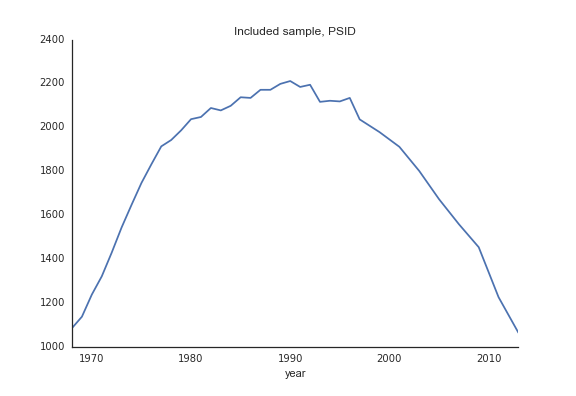
\includegraphics[width=\columnwidth]{PSID_sample}
\caption{Size of PSID estimation sample}
\label{fig:psid_sample}
\end{figure}


\footnote{To create the longitudinal data set from the PSID cross-sections, we
use the excellent \textit{PSIDtools} package \citep{Kohler2015}}. The main
variable of interest in the analysis is labour income, for which we use the
series of variables starting with \texttt{V74} in 1968\footnote{A complete list
of all variables used is available on
\href{https://github.com/nilshg/psidJulia/blob/master/create_panel.do}{my GitHub
page}.}. Hourly earnings are taken from the variable starting with \texttt{V337}
in 1968, while hours worked are taken from the variable starting with
\texttt{V47}. To extract the deterministic life-cycle component of the is 
modelled as a cubic polynomial in experience,
$g(\theta_t^0, \pmb{X}_{h,t}^i) = \theta_{0,t} + \theta_{1,t} h 
+ \theta_{2,t} h^2 + \theta_{3,t} h^3$. Labour market experience itself is 
constructed as potential experience from information on years of schooling. 
 \\
The BHPS data we are using comes from all available waves, covering the time 
period from 1992 to 2008\footnote{To merge the BHPS data across waves, we use 
code provided by \citet{Vandendriessche2015}.}. The raw data is then extended by
the derived current annual and net household variable data set provided by 
Horacio Levy and Stephen Jenkins, described in \citet{Jenkins2010}. This data set 
includes information on household income 
that takes into account various government taxes and transfers, both at the 
individual and the household level. For our purposes, we will use gross labour
income of the household, which is available in the original BHPS data set;
net household labour income, which considers taxes and tax credits, national
insurance contributions, and occupational pension contributions; and net 
household income, which adds investment income, pension income, and transfer
income to net labour income. These three variables can be seen to represent 
different levels of insurance available to the household: as taxes and (up to 
a point) National Insurance contributions in Britain are progressive, they reduce
the variability of the labour income process facing the household, while the
benefits system, which includes housing benefit, job seekers benefits, disability
insurance and various other payments, partially insures household income against
unemployment and other catastrophic shocks. It is therefore expected that these
measures of income imply less risk for the household than gross labour income,
an effect that we will try to quantify below. In addition, we are considering
the net \textit{equivalised} household income, which uses information on 
the size of the household to equivalise household income using the modified 
OECD scale. 
Potential labour market experience $h$ is calculated from information on the age
at which the household head finished either first or secondary education, which
other than in the PSID is available directly in the BHPS data set. 
As the time dimension is notably 
shorter than in the PSID, we only require households to be in the sample 
for five years, and consider up to ten lags for the covariances of residuals. 
While previous authors have highlighted the importance of higher order covariances
for identification of HIP processes, our sample sizes unfortunately are so small
that for some cohorts there are less than 10 observations at lags larger than
five, so that considering more lags is impossible. Figure \ref{fig:BHPS_sample_size}
shows the evolution of the sample size for the BHPS data set over time.

\begin{figure}
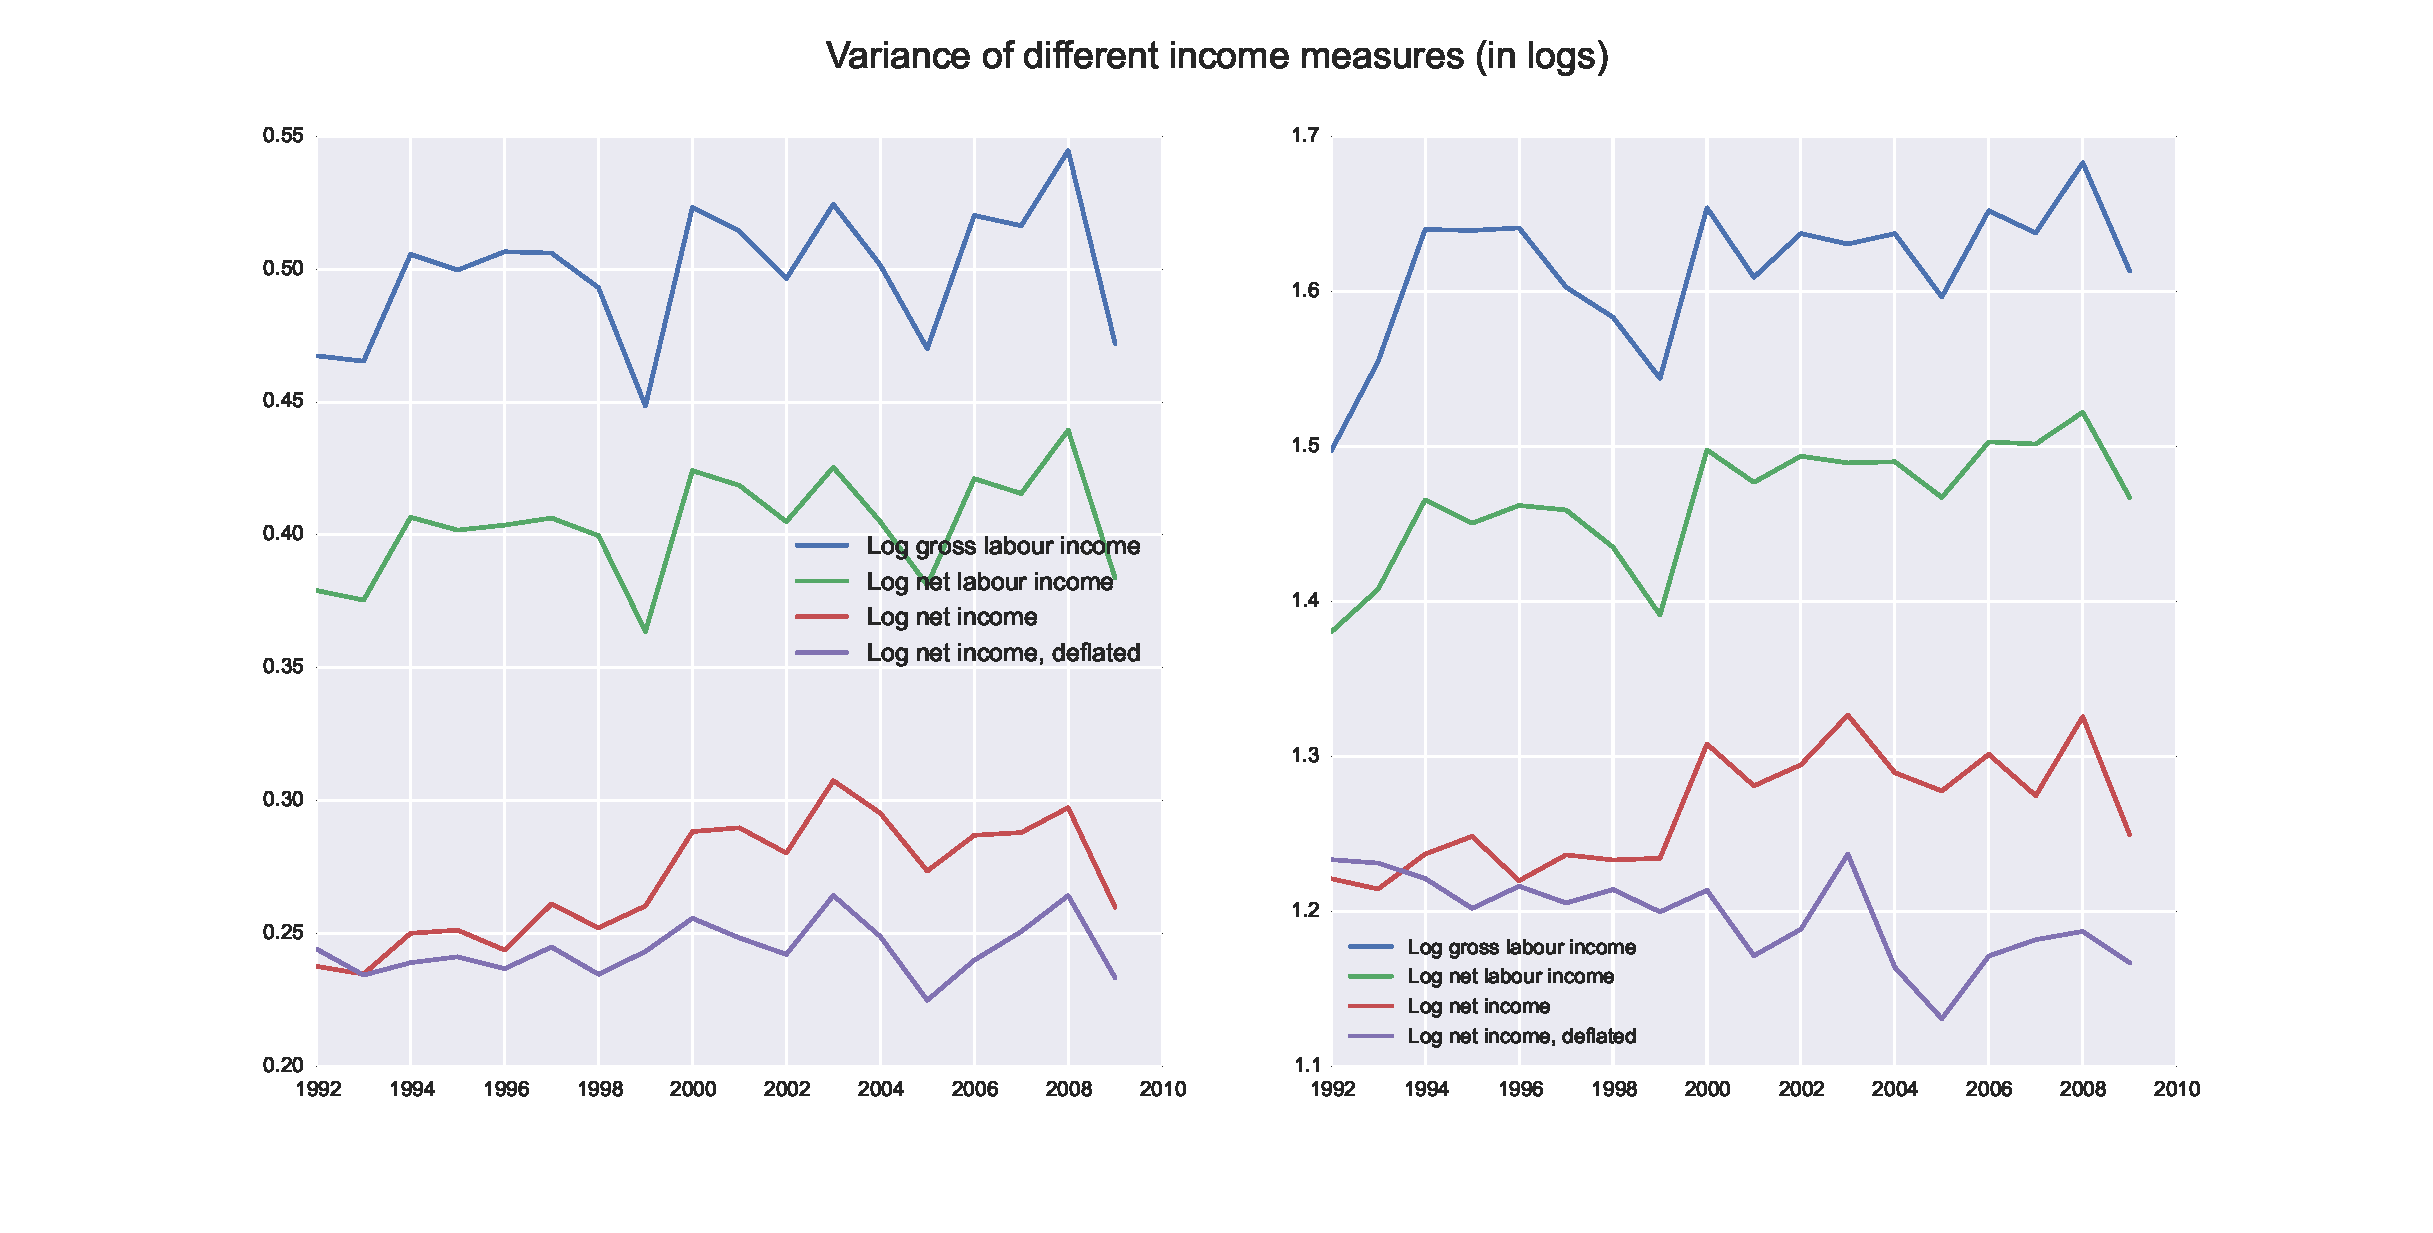
\includegraphics[width=\columnwidth]{BHPS_incvar}
\caption{Size of BHPS estimation sample}
\label{fig:BHPS_sample_size}
\end{figure}


As for the PSID, we obtain
income residuals by regressing each measure of income on a cubic polynomial 
in experience, which is constructed from the school leaving age (or further
education leaving age, where applicable). Figure \ref{fig:bhps_incvar} and
\ref{fig:psid_incvar} show trends in the variance and the inter-decile range,
two widely used measures of income dispersion, for our selected sample of households.
Both datasets exhibit considerable variation in the dispersion of income over 
the period under consideration, which motivates us to include time-varying
variances for transitory and permanent shocks in the estimation. \\
Figure \ref{fig:psid_residual_variance} shows the evolution of the residual
variance for our PSID sample, after fitting the cubic polynomial in experience.

\begin{figure}
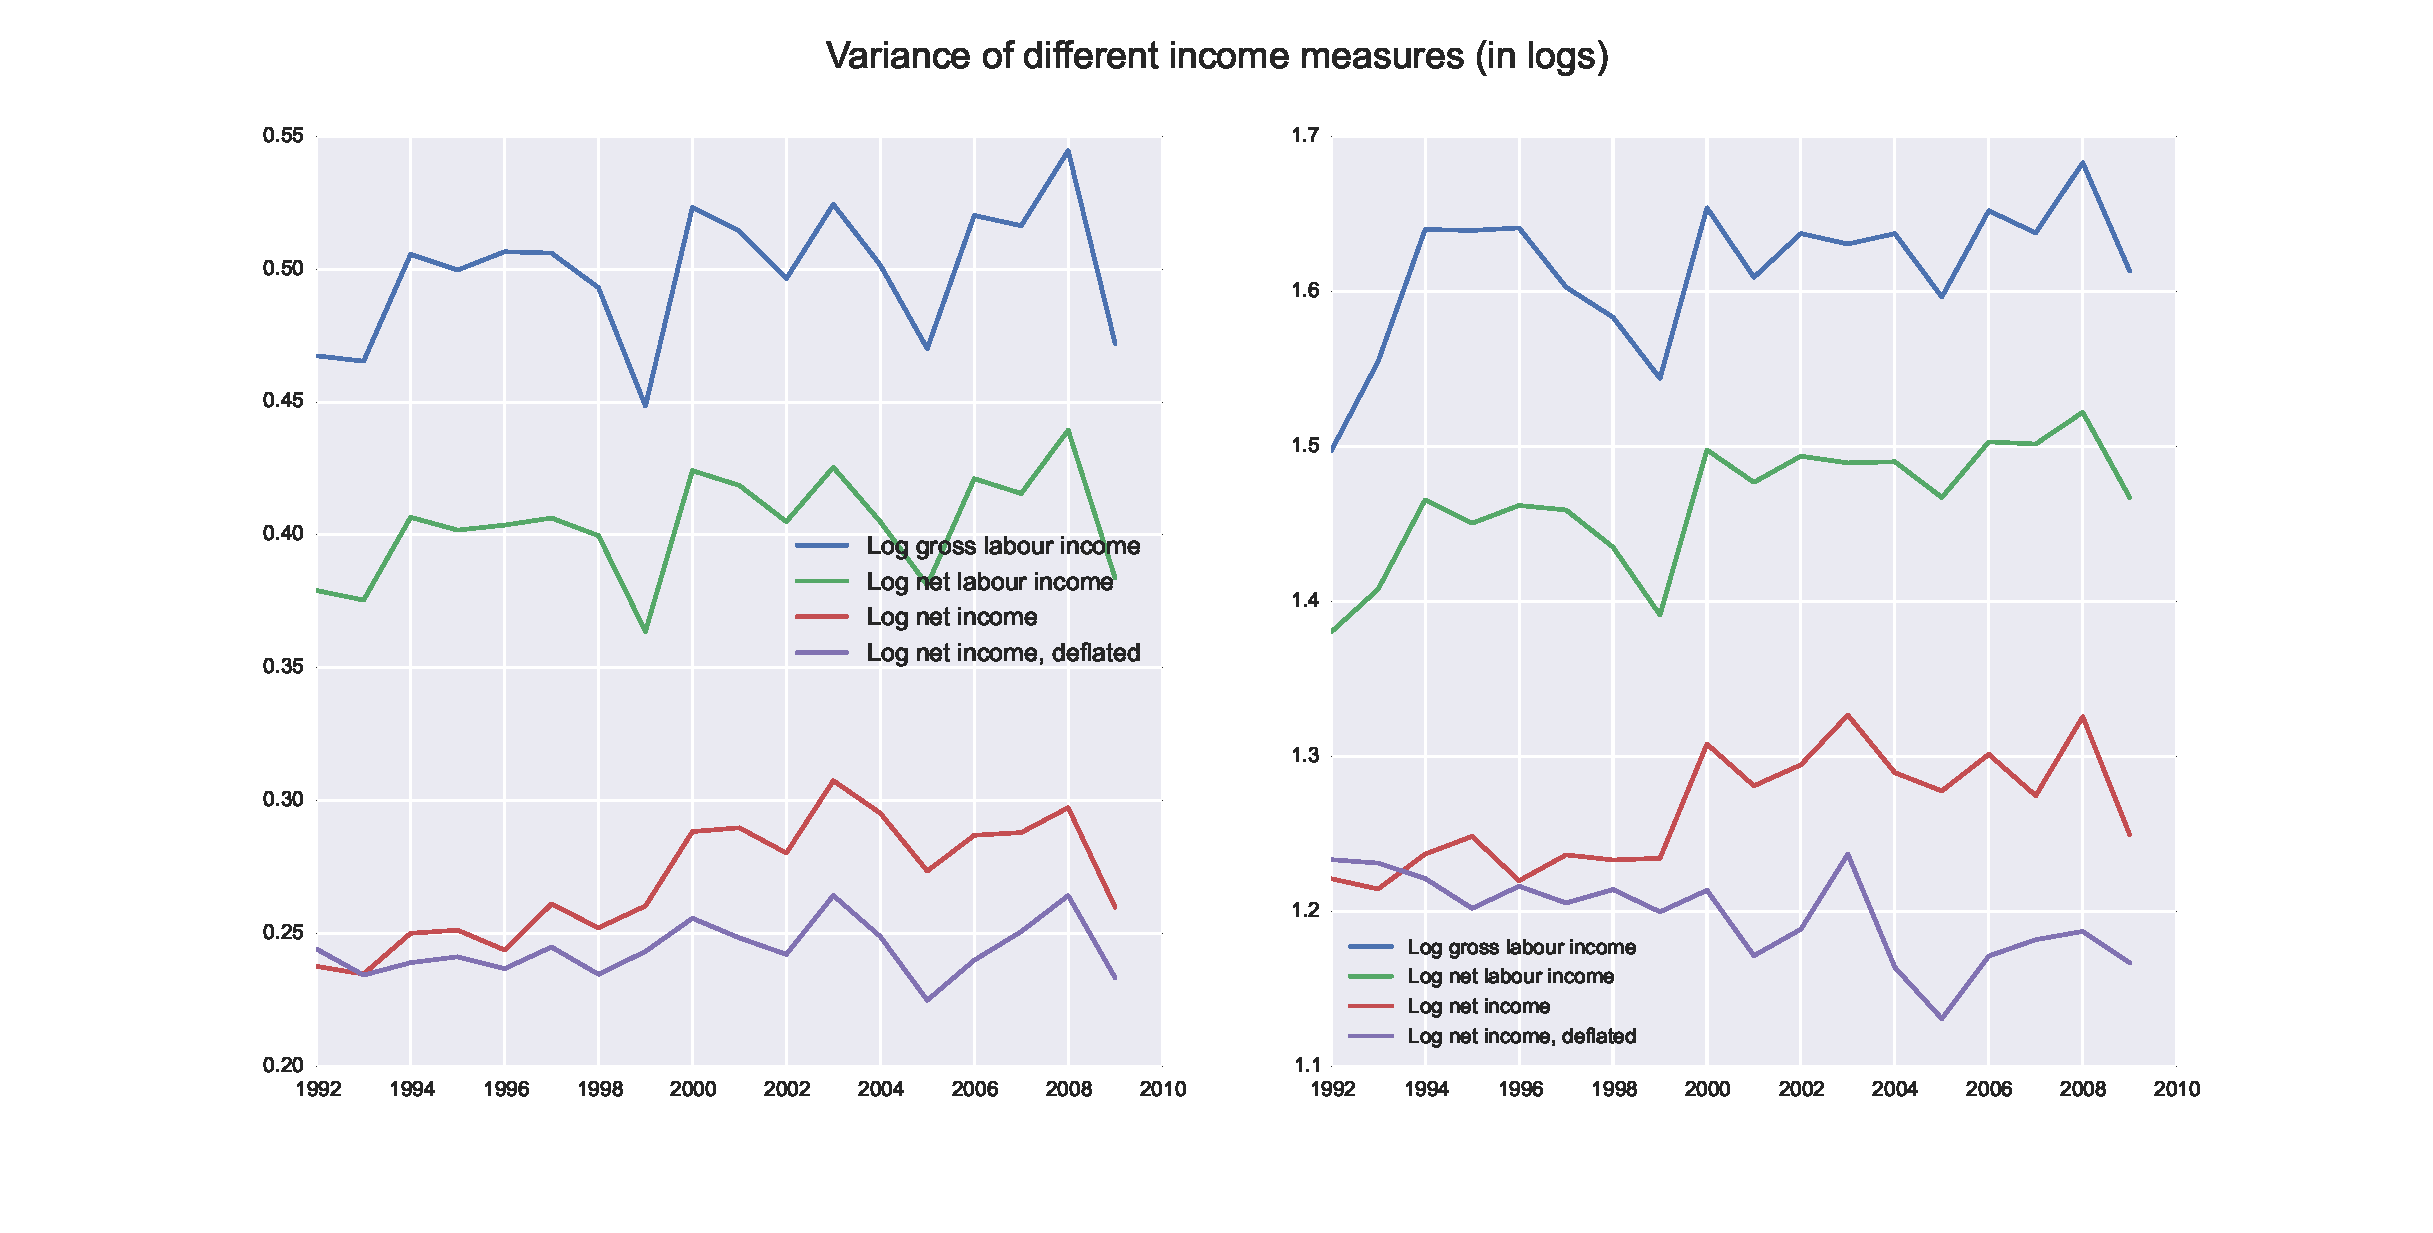
\includegraphics[width=\columnwidth]{BHPS_incvar}
\caption{Variance of log income and 90/10 percentile width for our sample of
BHPS households}
\label{fig:bhps_incvar}
\end{figure}

\begin{figure}
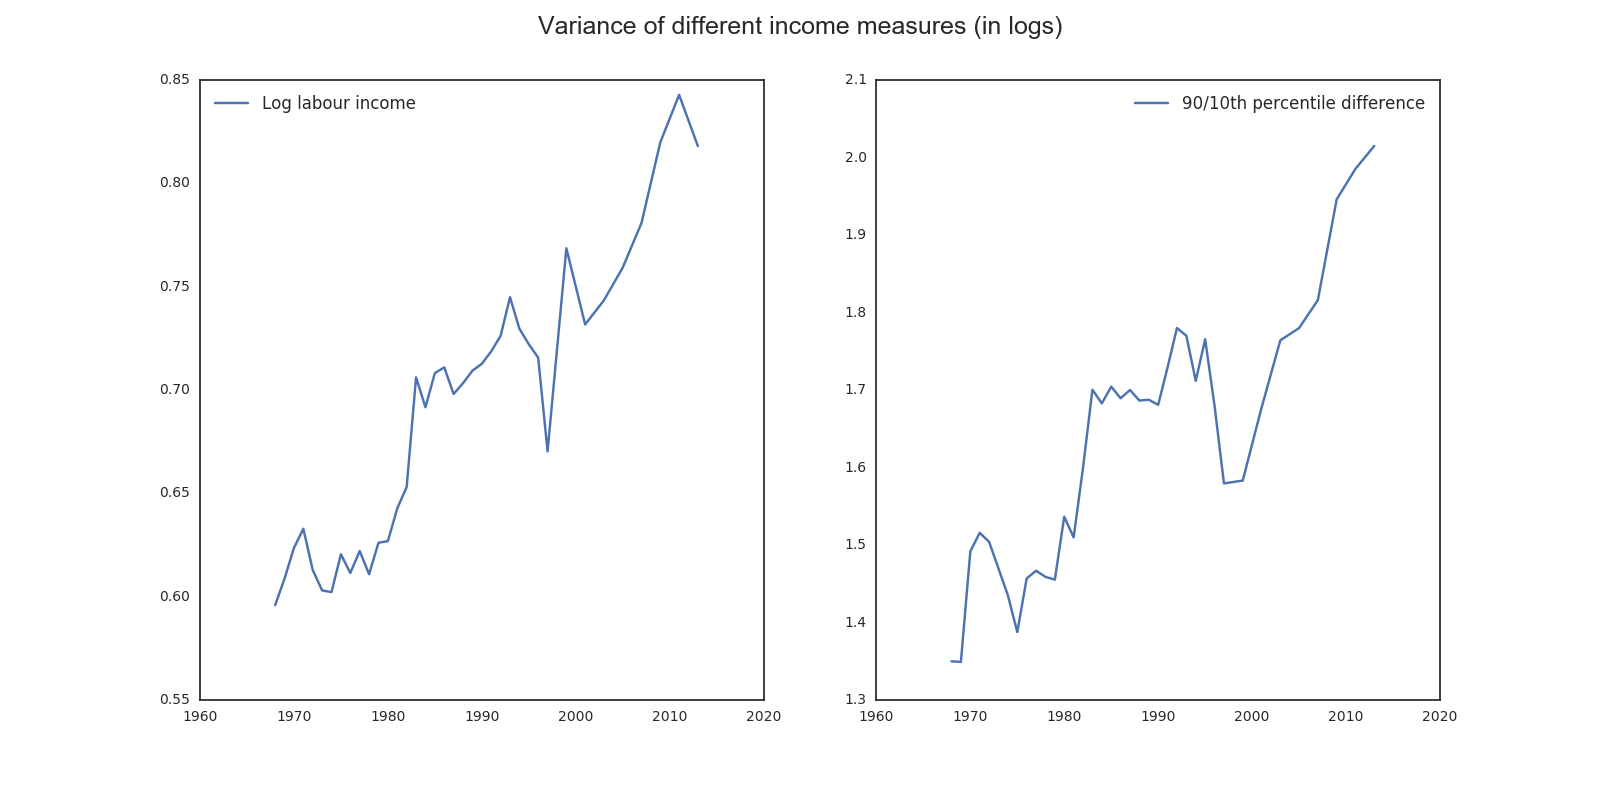
\includegraphics[width=\columnwidth]{PSID_incvar}
\caption{Variance of log income and 90/10 percentile width for our sample of
BHPS households}
\label{fig:psid_incvar}
\end{figure}

\begin{figure}
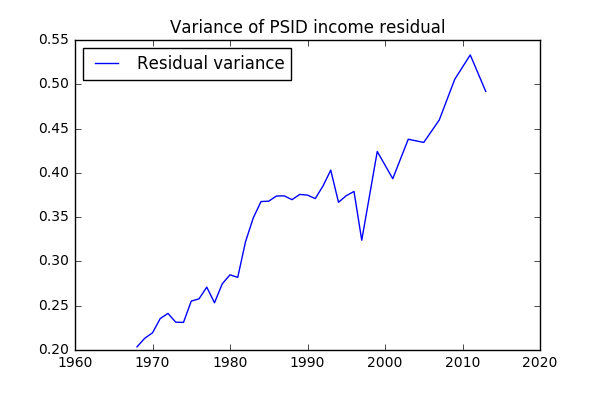
\includegraphics[width=\columnwidth]{PSID_residual_variance}
\caption{Variance of income residual from regression on cubic experience 
polynomial}
\label{fig:psid_residual_variance}
\end{figure}

\begin{figure}
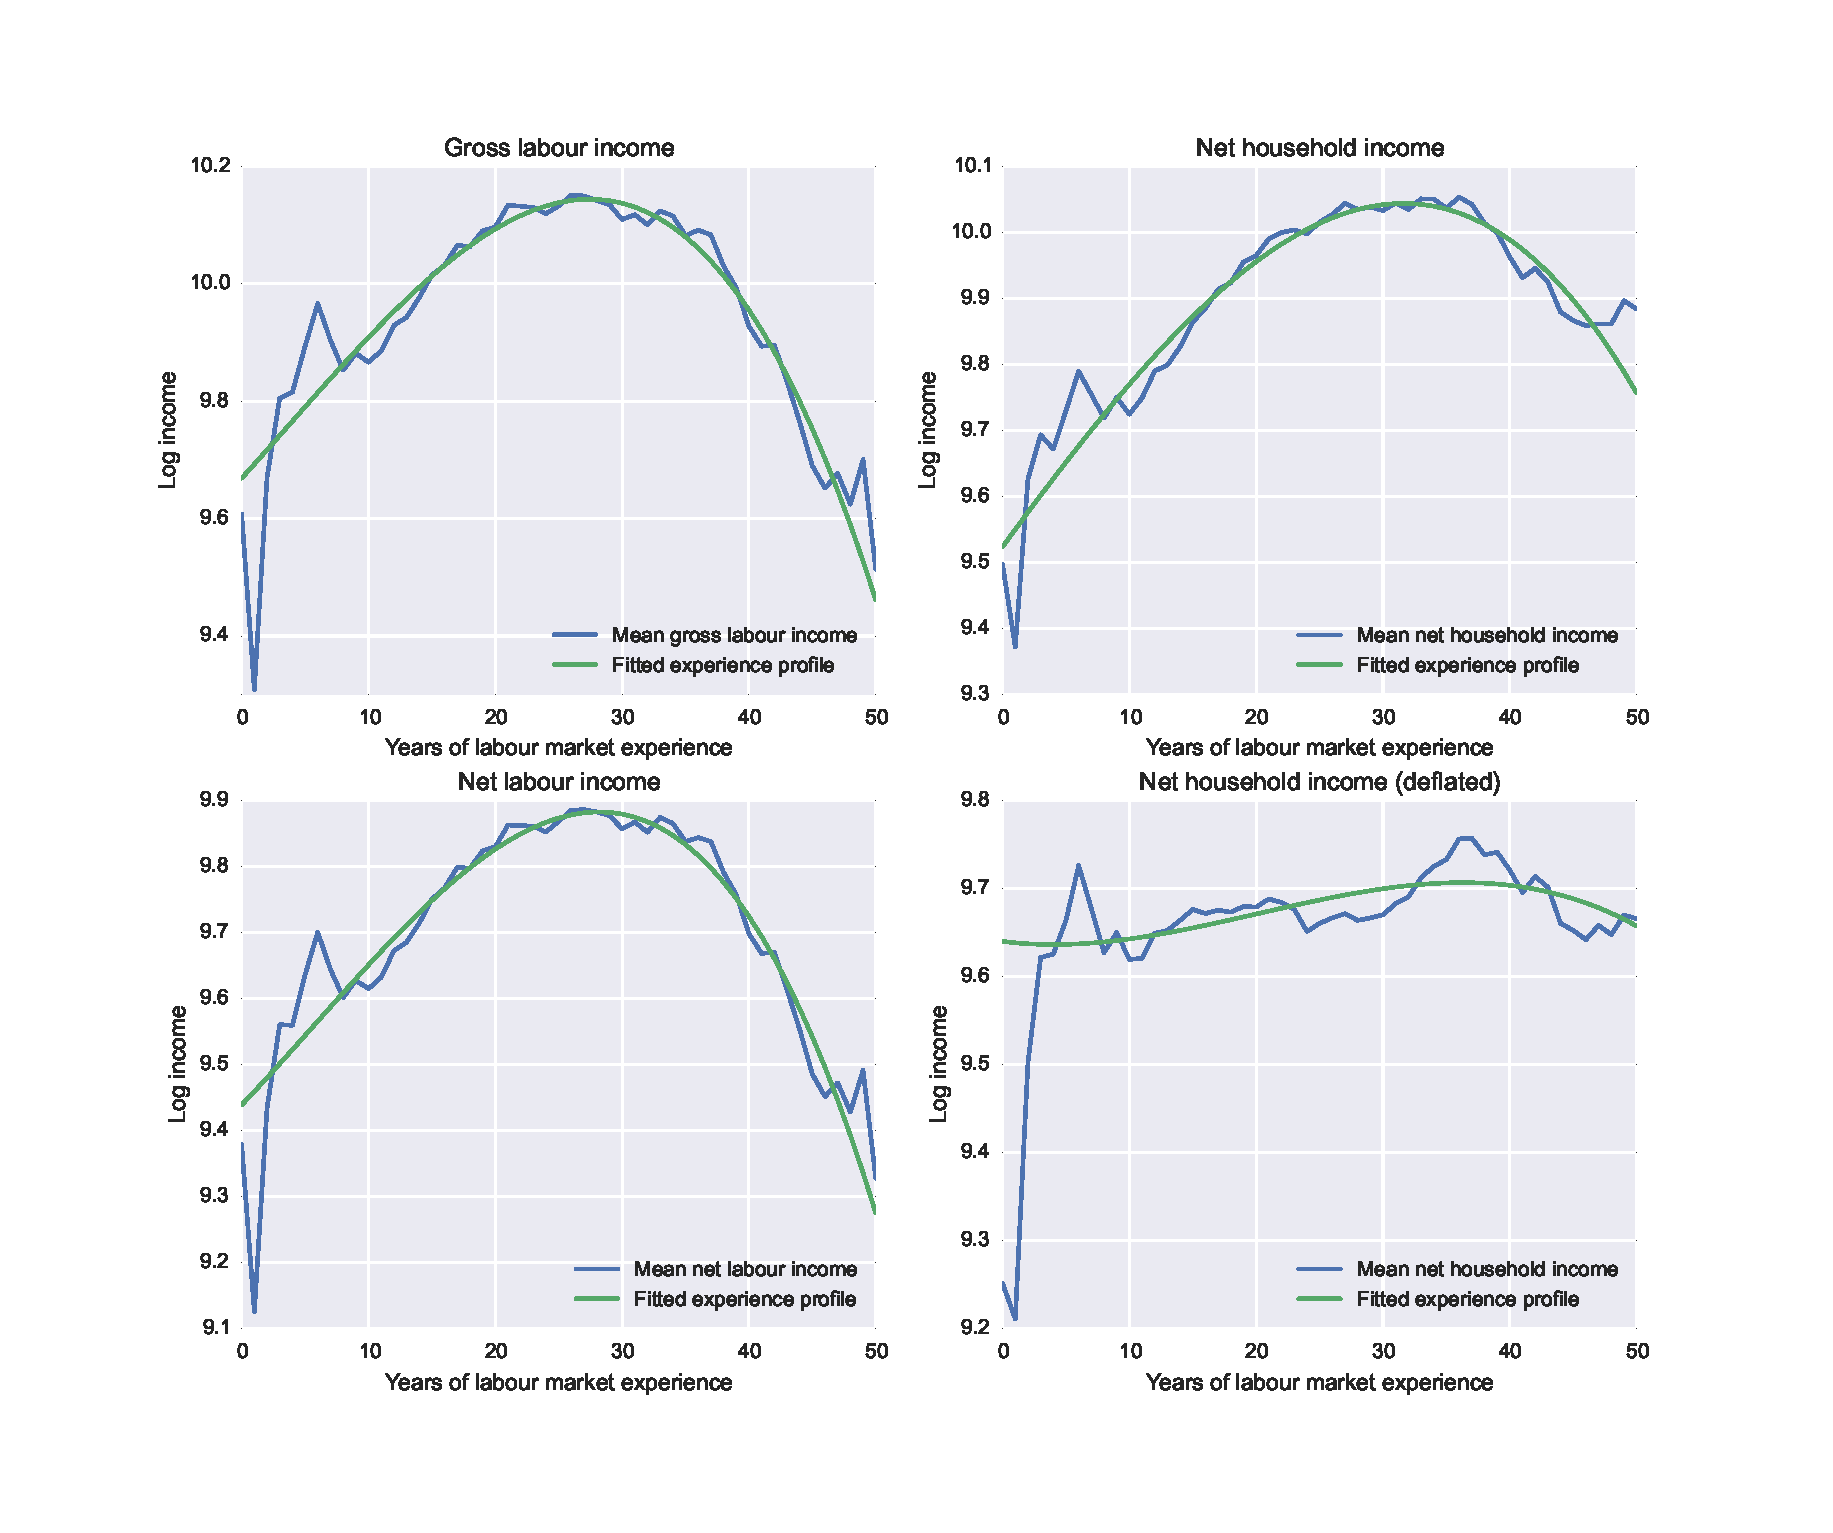
\includegraphics[width=\columnwidth]{BHPS_fitted_profiles}
\caption{Log mean income and fitted experience profiles for the BHPS 1992 
-- 2009}
\label{fig:bhps_profiles}
\end{figure}


\section{Results}
Table \ref{tab:PSID_results} displays the results for the PSID sample of households.
While the results can be considered to be qualitatively similar to those found
in \citet{Guvenen2009}, interestingly the estimated dispersion of individual-
specific growth rates declines from 0.00031 to 0.00025, a result that confirms
the same finding in \citet{Hryshko2012}. Furthermore, the difference in estimated
persistence for the HIP and RIP is much smaller than that reported by Guvenen,
and closer to the values found in \citet{Hryshko2012}\footnote{To ensure broad
correctness of our estimation procedure, we also downloaded and ran the code of
\citet{Guvenen2009} along with the original dataset used therein from the journal
website. Unfortunately, we were unable to replicate the results reported in the 
paper with this code; the results turn out to be much closer to our results reported
here. The author did not respond to repeated emails asking for clarification.}.
Table \ref{tab:BHPS_results} shows the results of estimating both RIP and HIP
processes on our sample of households from the BHPS, using the four different
income measures described previously. The results are largely unsurprising 
qualitatively, with the variance of persistent shocks declining from 0.1 for
the most volatile process (gross labour earnings) to 0.07 for net labour earnings,
to 0.027 for net household income. A similar pattern can be observed for the 
transitory shock, declining from 0.08 to 0.07 and 0.056, respectively. The 
estimates for the main parameter of interest, the cross-sectional dispersion 
in individual specific growth rates $\beta^i$ behaves accordingly, dropping from 
0.00032 (consistent with the findings for the main PSID sample in 
\citet{Guvenen2009}), to 0.00019 and 0.00011. Interestingly, some of the decrease
in the parameters that increase cross-sectional dispersion over the life-cycle
of a cohort is offset by a rise in the cross-sectional inequality in intercepts, 
$\var_{\alpha}$ rises from 0.036 in the gross labour income sample to 0.052 in 
the net household income sample. The persistence of 
The most peculiar set of estimates obtains for the deflated and equivalized
measure of net household income. Here, the RIP process shows a much lower persistence
as would be expected, while the variance of persistence shocks is surprisingly 
higher than in then in the raw measure of net household income. The results
for the HIP process indicate that the minimization routine hit the boundaries 
on both $\sigma^2_{\beta}$\footnote{Which actually has a lower bound of 1e-6, so 
is not exactly zero.} and $\cov(\alpha,\beta)$. A possible explanation for the 
large difference in results compared to all other income processes can be seen 
in figure \ref{fig:bhps_profiles}: as the equivalization largely removes the
hump-shape of the experience profile in the data, the fitted regression line
misses the sharp increase in income at the earliest stage of the life cycle, and
instead takes a flat shape over the entire range. This necessarily implies an
entirely different structure of residuals, with extremely large predicted residuals
for the first years of working life. Given this, we will not consider the estimates
for this process in the rest of this thesis\footnote{For the case of the HIP process 
this isn't actually a choice, as the estimated parameters for $\sigma^2_{\beta}$ and
$\cov{\alpha,\beta}$ imply a negative-definite variance covariance matrix for the
bivariate Normal distribution from which $\alpha$ and $\beta$ are drawn, making it
impossible to simulate an income distribution using these estimates.}.

\section{Discussion}
Our estimates point to substantial uncertainty over the correct HIP process, 
adding to a literature that has found vastly different estimates for all of the 
main parameters. Further, we have documented that even applying the same estimation
procedure to different subsamples of the same survey can deliver results that
differ markedly. Lastly, our estimates based on different income measures from 
the BHPS underscore the importance of partial insurance when trying to estimate
household income risk from the data. In the next chapter, we will explore the
quantitative implications of these differences for wealth accumulation in 
life-cycle models with incomplete markets.

\begin{table}%
\begin{tabular}{l|cccccc}
                     &$\rho$ & $\sigma^2_{\eta}$&$\sigma^2_{\varepsilon}$&$\sigma^2_{\alpha}$&$\sigma^2_{\beta}$&$\sigma_{\alpha \beta}$\\
\hline
\hline
\multicolumn{7}{c}{Restricted income process: $\sigma^2_{\beta} \stackrel{!}{=} 0$} \\
\hline \\
Gross labour income   & 0.925 &  0.045           &   0.135                &       0.0         &        --        &        --             \\
Net labour income     & 0.867 &  0.065           &   0.077                &       0.017       &        --        &        --             \\
Net household income  & 0.921 &  0.026           &   0.046                &       0.012       &        --        &        --             \\
Net household income (deflated) & 0.817 &  0.038 &   0.038                &       0.084       &        --        &        --             \\
\hline
\multicolumn{7}{c}{Heterogeneous income process; $\sigma^2_{\beta}$ unrestricted} \\
\hline
Gross labour income   & 0.719 &  0.106           &   0.080                &       0.036       &     0.00032      &       -0.51           \\
Net labour income     & 0.808 &  0.073           &   0.070                &       0.032       &     0.00019      &       -0.59           \\
Net household income  & 0.857 &  0.027           &   0.056                &       0.052       &     0.00011      &       -0.42           \\
Net household income (deflated) & 0.812 &  0.039 &   0.042                &       0.100       &        0.0       &       -1.0            \\
\hline
\end{tabular}
\caption{Results for the BHPS sample 1992--2008, different measures of household income}
\label{tab:BHPS_results}
\end{table}


\begin{table}%
\begin{tabular}{l|cccccc}
                    &$\rho$ & $\sigma^2_{\eta}$&$\sigma^2_{\varepsilon}$&$\sigma^2_{\alpha}$&$\sigma^2_{\beta}$&$\sigma_{\alpha \beta}$\\
\hline
\hline 
\multicolumn{7}{c}{Restricted income process: $\sigma^2_{\beta} \stackrel{!}{=} 0$} \\
1968-1996 sample & 0.932 &  0.010           &   0.036                &       0.084       &        --        &        --             \\
1968-2013 sample & 0.920 &  0.014           &   0.067                &       0.076       &        --        &        --             \\
1968-1986 sample & 0.960 &  0.015           &   0.061                &       0.058       &        --        &        --             \\
1987-2013 sample & 0.939 &  0.017           &   0.095                &       0.110       &        --        &        --             \\
\hline
\multicolumn{7}{c}{Heterogeneous income process: $\sigma^2_{\beta}$ unrestricted} \\
\hline
1968-1996 sample & 0.853 &  0.013           &   0.030                &   0.030           &     0.00031      &     --0.30            \\
1968-2013 sample & 0.839 &  0.017           &   0.064                &   0.047           &     0.00026      &     --0.32            \\
1968-1986 sample & 0.885 &  0.013           &   0.043                &       0.110       &      0.00028     &      -0.42            \\
1987-2013 sample & 0.854 &  0.032           &   0.085                &       0.097       &      0.00025     &      -0.31            \\
\hline
\end{tabular}
\caption{Results for the PSID, different sample periods.}
\label{tab:PSID_results}
\end{table}
